\documentclass[12pt,a4paper,oneside]{report}

\usepackage[utf8]{inputenc}
\usepackage[T1]{fontenc}
\usepackage[danish]{babel}

\usepackage[a4paper,width=150mm,top=30mm,bottom=25mm,headheight=2cm]{geometry}

\usepackage[style=authoryear,autocite=inline]{biblatex}
\bibliography{bib/references}

\usepackage{lastpage}
\usepackage{url}
\usepackage[hidelinks]{hyperref}

\usepackage{graphicx} % Import images
\usepackage{wallpaper}
\usepackage{pgfgantt} % Gantt Charts
\usepackage{float}

\usepackage[justification=centering]{caption}
\usepackage{subcaption}

\usepackage{color}

\usepackage{listings} % Code highlight
\definecolor{javared}{rgb}{0.6,0,0}
\definecolor{javagreen}{rgb}{0.25,0.5,0.35}
\definecolor{javapurple}{rgb}{0.5,0,0.35}
\definecolor{javadocblue}{rgb}{0.25,0.35,0.75}
 
\lstset{language=Java,
    basicstyle=\ttfamily\small,
    keywordstyle=\color{javapurple}\bfseries,
    stringstyle=\color{javared},
    commentstyle=\color{javagreen},
    morecomment=[s][\color{javadocblue}]{/**}{*/},
    numbers=left,
    numberstyle=\tiny\color{black},
    stepnumber=1,
    numbersep=10pt,
    tabsize=4,
    showspaces=false,
    showstringspaces=false,
    breaklines=true,
}

% Header style
\usepackage{fancyhdr}


\pagestyle{header-footer}

\makeatletter
\renewcommand\chapter{
    \if @openright
        \cleardoublepage
    \else
        \clearpage
    \fi

    \thispagestyle{header-footer}

    \global\@topnum\z@
    \@afterindentfalse
    \secdef\@chapter\@schapter
}
\makeatother

\usepackage{titlesec}
\definecolor{dtured}{cmyk}{0,.91,.72,.23}
\newcommand{\hsp}{\hspace{10pt}}
\titleformat{\chapter}[hang]{\Huge\bfseries}{\thechapter\hsp\textcolor{dtured}{|}\hsp}{0pt}{\Huge\bfseries}

\begin{document}
\section{Roskildeprojekt gruppe 18}
Formålet med vores kommende IT-system er at producere et billetsalgssystem, hvor man kan vælge produkt (partout, enkeltdag), se pris, ændre produkt og kan producere et salg af denne.

\section{Vision}
Vores vision er i dette projekt, at fremstille et system der kan holde til, at billetter bestilles i et stort omfang, og evt. i samme tidsramme uden at gå ned.\\

\section{Specifikationer}
Systemet skal være fuldendt funktionel under hele salgsperioden.
Typisk siges der at antal billetter mindst er på 100.000 stk, og dermed skal der være tilstrækkelige ressourcer til håndtering af billetterne.\\

\section{Forretningsregler}
Følgende er forretningsregler for Roskilde billetsalgssystem:
\begin{enumerate}
    \item Billetter refunderes ikke
    \item Billetter må gerne videresælges til andre, dog ikke over billettens pris inklusiv gebyr.
    \\
\end{enumerate}

\section{Kravspecifikationer}

\subsection{Kravsliste}

\begin{enumerate}
    \item Billetsalgssystemet skal sælge billetter til kunder.
    \item Billetsalgssystemet skal kunne udskrive billetter til kunder.
    \item Billetsalgssystemet skal kunne reservere en billet i maksimalt 15 minutter.
    \item Billetsalgssystemet skal kunne vise kundes aktuelle / tidligere køb.
    \item Billetsalgssystemet skal kunne modtage Visa/MasterCard/Dankort.
    \item Kunden skal kunne redigere billetkøbet.
    \item Kunden skal kunne vælge forskellige billetter
    \item Billetsalgssystemet skal maksimalt kunne sælge x-antal billetter.
    \item Skal kunne se antallet af solgte billetter (evt. mere statistik).
\end{enumerate}

\pagebreak

\subsubsection{MoSCoW}

\begin{tabular}{lll}
    \textbf{Mo} &   
    "Must have"                 &
    De mest vitale krav, vi ikke kan undgå. \\

    \textbf{S}  &   
    "Should have"               & 
    Vigtige krav, som ikke er vitale. \\

    \textbf{Co} &   
    "Could have"                & 
    The 'nice-to-haves' \\

    \textbf{W}  &   
    "Won’t have (this time)"    & 
    Things that provide little to no value you can give up on \\\\
\end{tabular}

\begin{tabular}{|p{0.2\textwidth}|p{0.75\textwidth}|}
    \hline
    Must have & \begin{itemize}
        \item 1. Billetsalgssystemet skal sælge billetter til kunder.
        \item 2. Billetsalgssystemet skal kunne udskrive billetter til kunder.
        \item 5. Billetsalgssystemet skal kunne modtage Visa/MasterCard/Dankort.
        \item 8. Billetsalgssystemet skal maksimalt kunne sælge x-antal billetter.
    \end{itemize} \\
    \hline
    Should have & \begin{itemize}
        \item 3. Billetsalgssystemet skal kunne reservere en billet i maksimalt 15 minutter.
        \item 4. Billetsalgssystemet skal kunne vise kundes aktuelle / tidligere køb.
        \item 6. Kunden skal kunne redigere billetkøbet.
    \end{itemize} \\
    \hline
    Could have & \begin{itemize}
        \item 7. Kunden skal kunne vælge forskellige billetter
        \item 9. Skal kunne se antallet af solgte billetter (evt. mere statistik).
    \end{itemize} \\
    \hline
    Won't have (this time) & \\
    \hline
\end{tabular}

\section{Use Case-diagram}
\begin{figure}[H]
    \begin{center}
        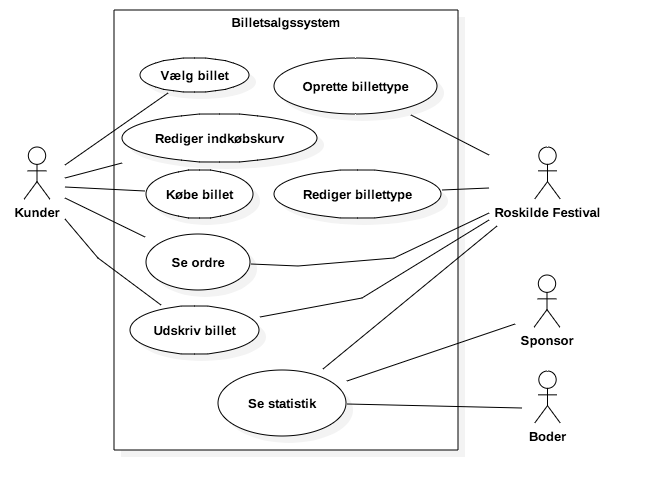
\includegraphics[width=1\textwidth]{UseCaseDiagram.png}
    \end{center}
\end{figure}

\section{Domænemodel}
\begin{figure}[H]
    \begin{center}
        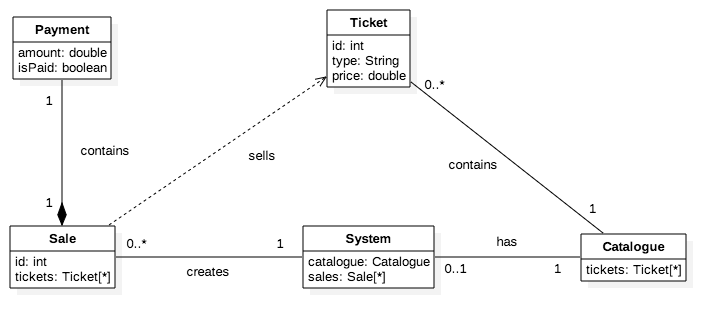
\includegraphics[width=1\textwidth]{Domainmodel.png}
    \end{center}
\end{figure}

\section{Klassediagram}
\begin{figure}[H]
    \begin{center}
        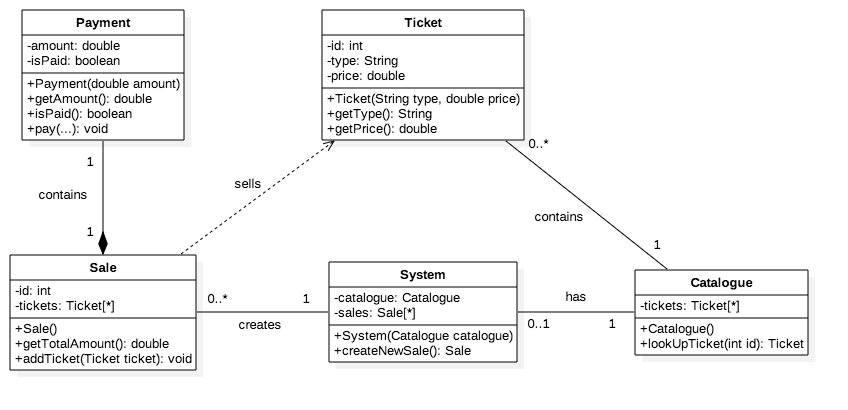
\includegraphics[width=1\textwidth]{Klassediagram.png}
    \end{center}
\end{figure}

\end{document}
